%!TEX TS-program = xelatex
%!TEX encoding = UTF-8 Unicode

\documentclass[11pt,tikz,border=1]{standalone}
\usetikzlibrary{calc,positioning}

\begin{document}
  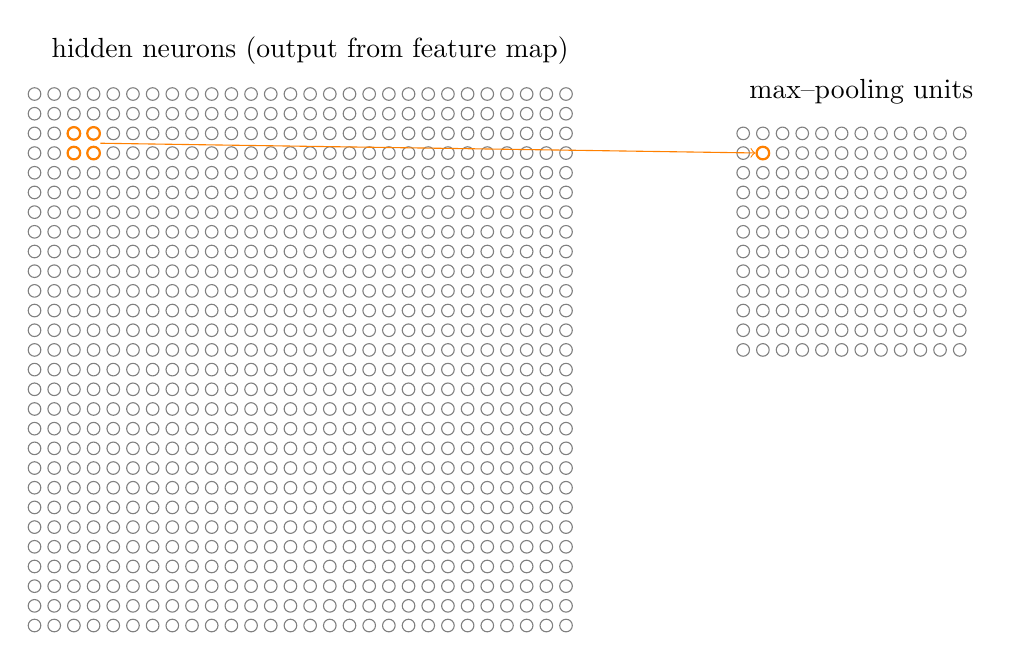
\begin{tikzpicture}[
    neuron/.style={circle,draw,inner sep=0pt,minimum size=1.6mm}
    ]

    \foreach \x in {0,...,27}
      \foreach \y in {0,...,27}
        \node (x\x y\y) [neuron,gray] at (\x * 0.25,\y * 0.25) {};

    \node [above] at (3.5,7) {hidden neurons (output from feature map)};

    \foreach \x in {0,...,11}
      \foreach \y in {0,...,11}
        \node (m\x n\y) [neuron,gray] at (\x * 0.25 + 9, \y * 0.25 + 3.5) {};

    \node [above] at (10.5, 6.5) {max--pooling units};

    \node(hidden) [neuron,orange,thick] at (m1n10) {};

    \foreach \x in {2,3}
      \foreach \y in {24,25}
        \node (a\x b\y) [neuron,orange,thick] at (\x * 0.25,\y * 0.25) {};

    \coordinate(p) at ($(x3y24.east)!0.5!(x3y25.east)$);
    \draw[->,orange] (p) to (hidden);

  \end{tikzpicture} 
\end{document}
